% ARR 2025 submission — uses the standard ACL template
\documentclass[11pt]{article}

% ACL style
\usepackage[hyperref]{acl}
\usepackage{times}
\usepackage{latexsym}
\usepackage[T1]{fontenc}
\usepackage[utf8]{inputenc}
\usepackage{microtype}
\usepackage{inconsolata}

% Additional packages
\usepackage{amsmath,amssymb}
\usepackage{graphicx}
\graphicspath{{figures/}}
\usepackage{booktabs}
\usepackage{multirow}
\usepackage{subcaption}
\usepackage{xcolor}
\usepackage{enumitem}
% \usepackage{tikz}  % uncomment if using TikZ figures

% For anonymous ARR submission: comment out \aclfinalcopy
% \aclfinalcopy  % uncomment for camera-ready
%\def\aclpaperid{XXX}


\newcommand{\modelsmall}{Qwen2.5-3B}
\newcommand{\modelmed}{Qwen2.5-7B}
\newcommand{\modellarge}{Qwen2.5-14B}
\newcommand{\modelphi}{Phi-3.5-mini}

\title{Thinking It's Wrong, Saying It's Right: \\ Hidden Error Awareness in Chain-of-Thought Reasoning}

\author{
  Anonymous ARR Submission
}

\begin{document}
\maketitle

% ============================================================
\begin{abstract}
Chain-of-thought (CoT) reasoning is widely assumed to reflect a language model's internal computation.
We show this assumption is wrong: a simple linear probe on hidden states predicts whether a CoT trace will reach the correct answer with up to 0.95 AUROC, while the model's own verbalized confidence is nearly uninformative (4.55/5 for wrong traces vs.\ 4.87/5 for correct).
The error signal is detectable from the \textit{very first} reasoning step (AUROC 0.79), before any visible mistake has been generated.
We observe this phenomenon across two model families (Qwen, Phi) and scales from 1.5B to 72B parameters---the 72B model achieves the \textit{highest} probe accuracy (0.98 AUROC)---though the signal's temporal profile varies: smaller models ``know immediately'' while larger models accumulate the signal gradually.

Can this internal error awareness be leveraged for self-correction?
We test four intervention strategies---activation steering, probe-guided best-of-N, self-correction, and activation patching---and find that \textbf{none meaningfully improve accuracy}.
Self-correction \textit{degrades} performance ($-3\%$); patching correct hidden states into wrong traces \textit{destroys} output quality (accuracy $\to 0\%$).
The error representation is \textbf{diagnostic, not causal}: it reflects awareness of reasoning quality without constituting a lever that can redirect computation.
The sole effective application is \textit{selective routing}---using the probe to flag likely errors and routing only those to an external verifier---achieving +8\% accuracy at 40\% of full verification cost.

Our findings expose a fundamental asymmetry in LLM reasoning: models internally detect their errors but cannot act on this knowledge.
We term this \textit{hidden error awareness} and argue it has direct implications for CoT interpretability, self-improvement, and the design of inference-time compute strategies.
\end{abstract}

% ============================================================
\section{Introduction}
\label{sec:intro}

Chain-of-thought (CoT) prompting \cite{wei2022chain} has become the dominant paradigm for eliciting complex reasoning from large language models (LLMs).
A tacit assumption underlies this paradigm: the generated reasoning trace faithfully reflects the model's internal computation.
If the text says ``Step 1: $3 \times 5 = 15$,'' the model presumably computed this multiplication and will build on it.
Recent work has begun to question this assumption from the perspective of text-level interventions \cite{turpin2024language, lanham2023measuring}, but a direct comparison between \textit{what models say} and \textit{what they internally represent} during reasoning has been lacking.

\begin{figure*}[t]
\centering
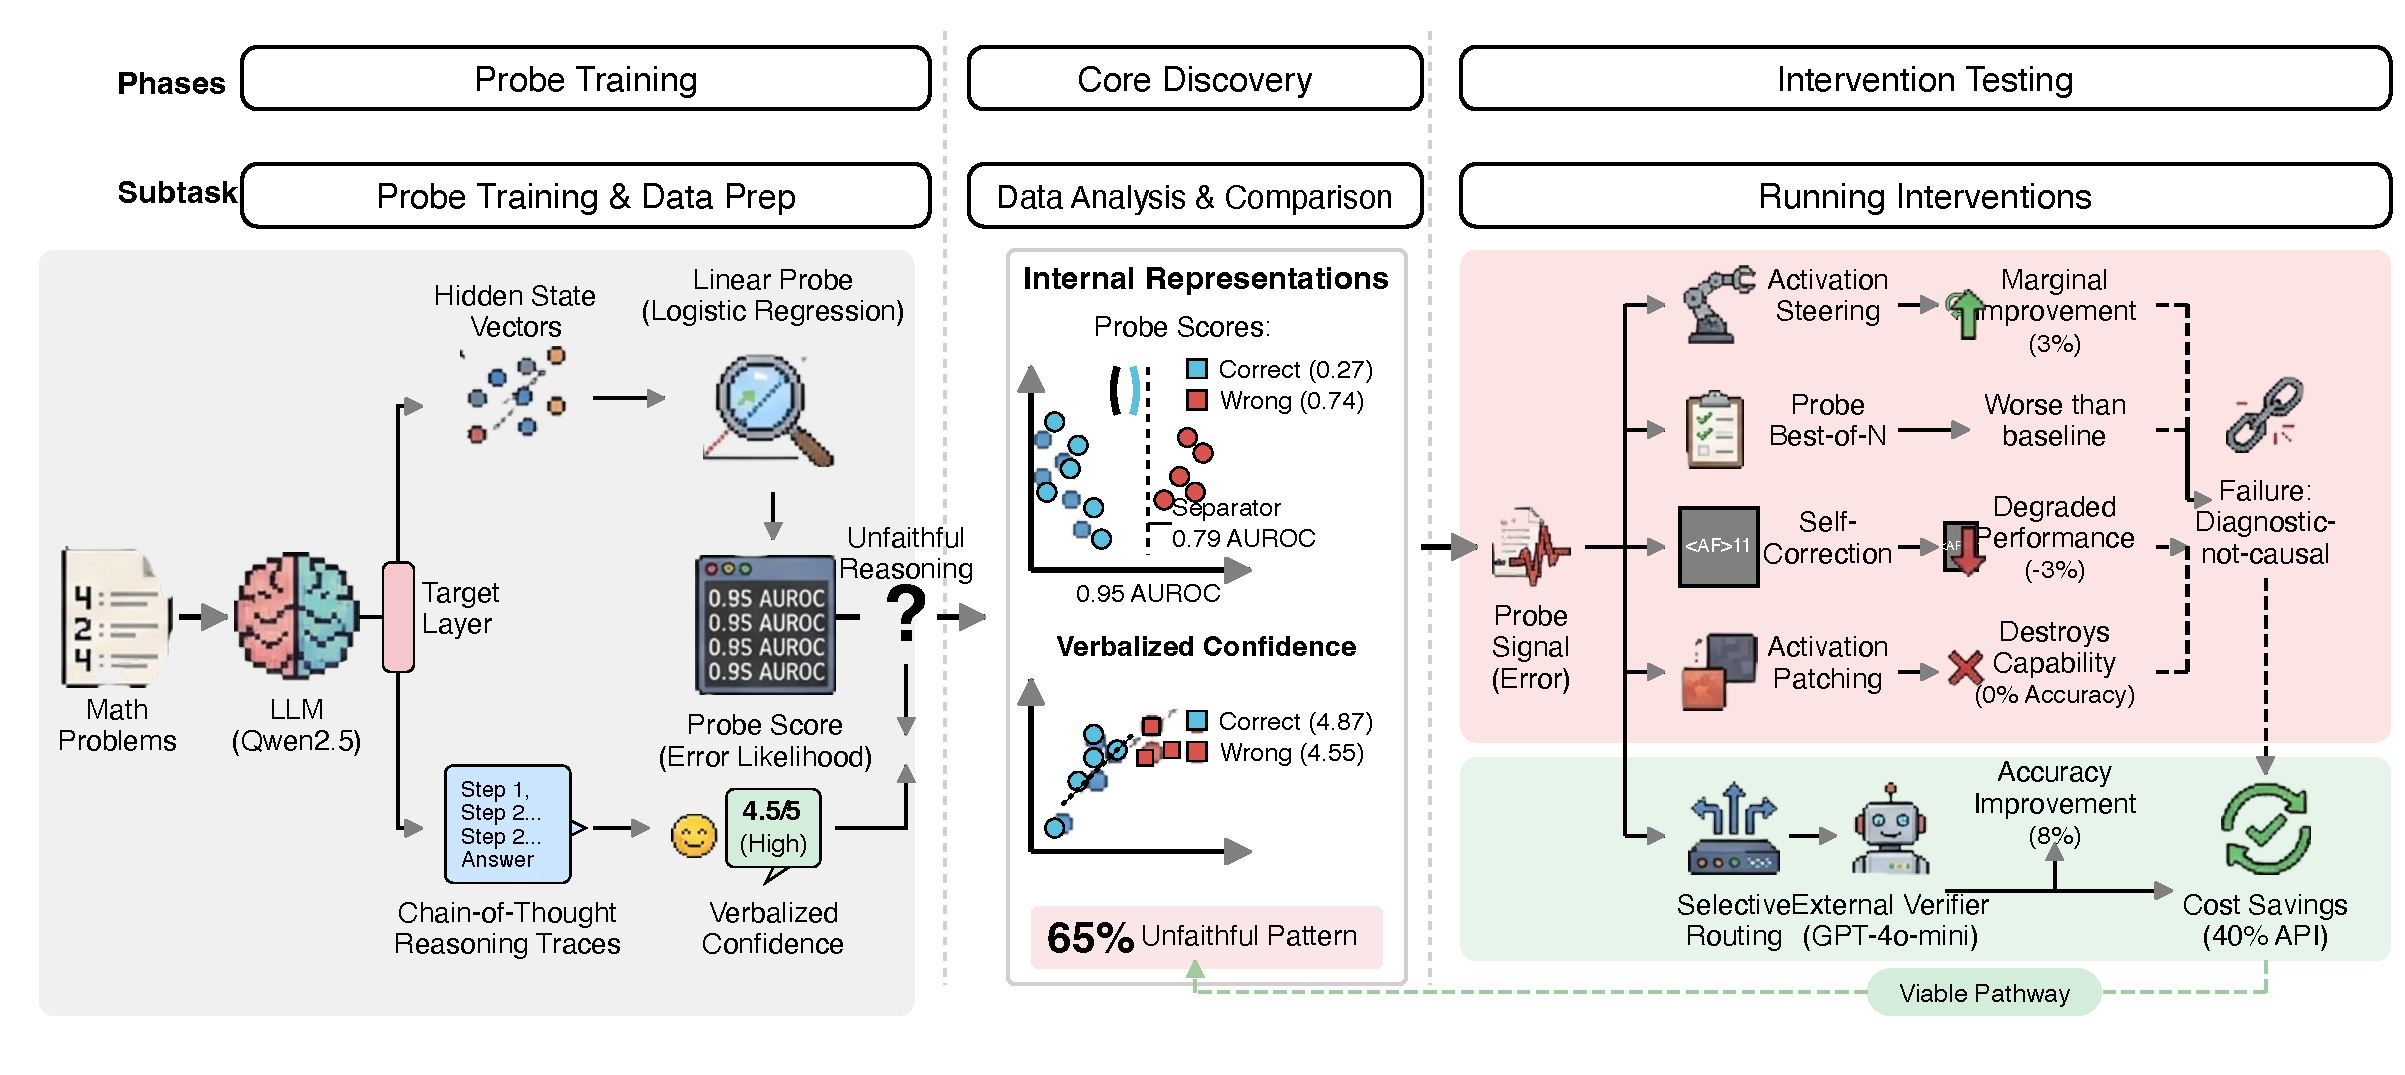
\includegraphics[width=\textwidth]{fig_overview_autofigure.pdf}
\caption{\textbf{Overview.} \textbf{(a)}~We extract hidden-state vectors from each CoT step and train a linear probe to predict error. \textbf{(b)}~Probe scores cleanly separate correct from wrong traces (AUROC\,=\,0.95), while verbalized confidence is near-identical---65\% of wrong traces exhibit \emph{hidden error awareness}. \textbf{(c)}~Four internal interventions fail to leverage this signal; only external selective routing succeeds (+8\% at 40\% cost).}
\label{fig:overview}
\end{figure*}

We provide this comparison through a simple experiment: training linear probes on hidden states extracted during CoT generation (Figure~\ref{fig:overview}).
Our findings are organized around three questions:

\vspace{2pt}
\noindent\textbf{Q1: Do models internally detect their reasoning errors?}
Yes. A logistic regression probe on a single hidden-state vector achieves 0.95 AUROC for predicting trace correctness, far exceeding verbalized confidence (0.67 AUROC), self-consistency (0.82), and CCS \cite{burns2023discovering} (0.72).
The signal is present from the \textit{very first} reasoning step (0.79 AUROC), before any error appears in the text (\S\ref{sec:detection}--\ref{sec:early}).

\vspace{2pt}
\noindent\textbf{Q2: Does the text reflect this internal knowledge?}
No. Wrong traces express verbalized confidence of 4.55/5, barely distinguishable from correct traces (4.87/5).
Only 1\% of traces contain hedging language.
Fully 65\% of wrong traces simultaneously show high confidence and high probe error scores---a phenomenon we term \textit{hidden error awareness} (\S\ref{sec:unfaithful}).

\vspace{2pt}
\noindent\textbf{Q3: Can this signal improve reasoning?}
Not through internal means. Four intervention strategies---activation steering, probe-guided best-of-N, self-correction, and activation patching---all fail.
Patching correct hidden states into wrong traces \textit{destroys} output (accuracy $\to 0\%$), revealing that the error signal is a diagnostic readout, not a causal lever (\S\ref{sec:interventions}).
However, using the probe to \textit{selectively route} likely errors to an external verifier achieves +8\% accuracy at 40\% of the cost of universal verification (\S\ref{sec:routing}).

\vspace{4pt}
These results expose a fundamental asymmetry: LLMs can detect their reasoning errors but cannot act on this knowledge.
This has implications for CoT interpretability \cite{turpin2024language}, the limits of self-correction \cite{huang2024large}, and the design of inference-time compute strategies.

% ============================================================
\section{Related Work}
\label{sec:related}

\paragraph{CoT Faithfulness.}
Several works question whether CoT reasoning faithfully reflects model computation.
\citet{turpin2024language} show that CoT explanations can be steered by irrelevant features (e.g., suggested answers in the prompt), and \citet{lanham2023measuring} find that perturbing or truncating CoT steps often does not change the final answer, suggesting answers may be reached independently of the stated reasoning.
These studies diagnose unfaithfulness via \textit{behavioral} interventions on the text.
Our work provides a complementary \textit{representational} perspective: we directly compare what hidden states encode with what the text expresses, revealing a quantifiable gap.

\paragraph{Probing Internal Representations.}
Linear probing has a long history in NLP \cite{belinkov2022probing,alain2017understanding}.
Most relevant to our work: \citet{burns2023discovering} discover ``truth directions'' in hidden states via unsupervised CCS; \citet{azaria2023internal} train classifiers on internal states to detect falsehoods; and \citet{kadavath2022language} show LLMs can calibrate uncertainty.
\citet{li2024inference} use probes for inference-time intervention, and \citet{zou2023representation} introduce representation engineering for reading and controlling model behavior.
Concurrent work by \citet{zhang2025reasoning} probes hidden states in reasoning models for self-verification, using the signal for early exit and best-of-N selection.
Our work differs in three respects: (1) we study standard CoT models rather than dedicated reasoning models; (2) we systematically test and \textit{falsify} the hypothesis that the signal can improve reasoning via four intervention strategies; and (3) we show the signal is present from the \textit{very first} reasoning step, before any error appears in text.
The negative intervention results are our central contribution---they reveal a fundamental asymmetry that verification-focused work does not address.

\paragraph{Self-Correction and Causal Analysis.}
\citet{huang2024large} find that intrinsic self-correction (without external feedback) remains limited, and \citet{kamoi2024can} show LLMs cannot reliably identify their own errors.
Our work reaches the same conclusion from a mechanistic perspective: even when models \textit{internally represent} error signals, they cannot leverage them.
Our activation patching experiments build on causal mediation analysis \cite{vig2020investigating,meng2022locating,geiger2024finding}, extending it from factual recall to multi-step reasoning.

\paragraph{Inference-Time Compute and Routing.}
Best-of-N sampling \cite{lightman2024lets}, majority voting \cite{wang2023selfconsistency}, and verifier-guided decoding \cite{cobbe2021training} improve reasoning at inference time but apply uniformly to all problems.
Process reward models (PRMs) score individual reasoning steps but require step-level human labels for training.
Recent routing frameworks use output confidence \cite{shen2025sater} or learned routers to direct queries to appropriate models.
Our probe is complementary: it requires only binary outcome labels (50 problems suffice), uses \textit{hidden states} rather than output confidence as the routing signal, and is most effective for \textit{triage}---identifying which problems warrant expensive verification---rather than selection among candidates or model routing.

% ============================================================
\section{Probe-Based Error Detection}
\label{sec:detection}

\subsection{Method}

Given a language model $\mathcal{M}$ with $L$ layers, we extract the hidden state $\mathbf{h}^{(l)}_T \in \mathbb{R}^d$ at layer $l$ and the last token position $T$ of a complete CoT trace.
We train a logistic regression classifier:
\begin{equation}
p(\text{error} \mid \mathbf{h}) = \sigma(\mathbf{w}^\top \mathbf{h} + b)
\end{equation}
where $\mathbf{h}$ is the standardized hidden state (zero mean, unit variance per dimension), and the label is 1 if the trace leads to an incorrect final answer.

\paragraph{Training.}
We use 100 problems from MATH-500 \cite{hendrycks2021math} for training (disjoint from all evaluation sets), generating one greedy CoT trace per problem.
We train separate probes at each candidate layer and select the best by 5-fold cross-validated AUROC.
The probe requires only standard logistic regression with $L_2$ regularization ($C=0.1$); no hyperparameter search is performed beyond layer selection.

\subsection{Results}

\begin{table}[t]
\centering
\small
\begin{tabular}{lcccc}
\toprule
\textbf{Model} & \textbf{Acc} & \textbf{Layer} & \textbf{CV AUROC} & \textbf{Trace AUROC} \\
\midrule
\modelsmall & 0.53 & 27 & 0.953 & 0.956 \\
Qwen2.5-1.5B & 0.35 & 27 & 0.918 & 0.724 \\
\modelphi & 0.39 & 8 & 0.936 & --- \\
\modelmed & 0.62 & 16 & 0.669 & 0.737 \\
\modellarge & 0.65 & 39 & 0.762 & --- \\
\midrule
Qwen2.5-32B & 0.53 & 32 & 0.956 & --- \\
Qwen2.5-72B & 0.41 & 64 & \textbf{0.977} & --- \\
\bottomrule
\end{tabular}
\caption{Probe error detection across models. CV AUROC is 5-fold cross-validation on training data; Trace AUROC is evaluation on held-out problems. All probes are simple logistic regression on the last token's hidden state at the best layer.}
\label{tab:probe_detection}
\end{table}

Table~\ref{tab:probe_detection} shows that linear probes detect errors across all models tested.
The probe achieves $>$0.9 AUROC for five of seven models (3B, 1.5B, Phi-3.5-mini, 32B, 72B), demonstrating that a single logistic regression on one hidden-state vector is a remarkably effective error detector \textit{even at 72B scale}.
The signal is weaker for the 7B and 14B models (0.669 and 0.762); notably, both the 32B (0.956) and 72B (0.977) models recover high probe accuracy, suggesting the intermediate-scale dip reflects training dynamics rather than a fundamental scaling limitation (\S\ref{sec:discussion}).
Figure~\ref{fig:layers} shows probe AUROC across layers; upper layers (70--85\% depth) consistently provide the strongest signal.

\begin{figure}[t]
\centering
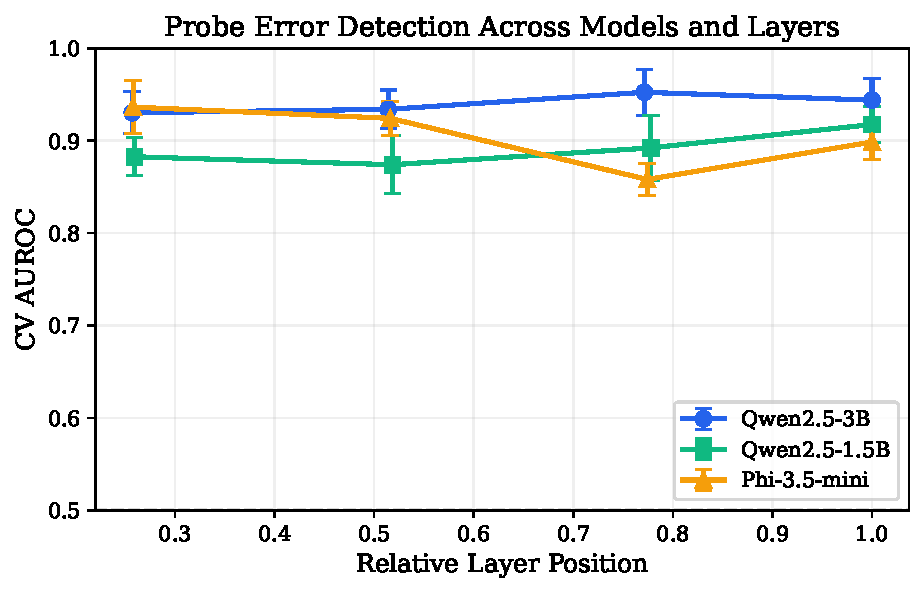
\includegraphics[width=\columnwidth]{fig2_probe_auroc_layers.pdf}
\caption{Probe AUROC across layers for multiple models. Upper layers (70--85\% depth) consistently achieve the best error detection, suggesting the error signal is encoded in the model's higher-level representations.}
\label{fig:layers}
\end{figure}

\paragraph{Comparison with baselines.}
Table~\ref{tab:baselines} compares our probe with established error detection methods on 200 held-out MATH-500 problems.

\begin{table}[t]
\centering
\small
\begin{tabular}{lcc}
\toprule
\textbf{Method} & \textbf{AUROC} & \textbf{Cost} \\
\midrule
Hidden State Probe (ours) & \textbf{0.953} & 1 fwd pass \\
Self-Consistency ($N$=5) & 0.823 & 5$\times$ gen \\
CCS \cite{burns2023discovering} & 0.718 & 1 fwd pass \\
$P$(\text{True}) & 0.721 & 1 query \\
Verbalized Confidence & 0.674 & 1 query \\
Sequence Log-prob & 0.676 & free \\
\bottomrule
\end{tabular}
\caption{Error detection comparison. Our probe substantially outperforms all baselines at minimal compute cost.}
\label{tab:baselines}
\end{table}

The probe outperforms all baselines, including self-consistency (which requires 5$\times$ the generation compute) and CCS (which uses the same hidden states but in an unsupervised manner).
Ablation studies confirm the signal is linearly encoded (linear probe 0.955 AUROC vs.\ MLP 0.944, random forest 0.893), stable with minimal data (20 problems yield 0.956), and strongest in upper layers (70--85\% depth).

\paragraph{Difficulty control.}
A key concern is whether the probe merely learns problem difficulty rather than trace-specific error signals.
We test this with a \textit{within-problem} experiment: for 50 problems, we generate 5 traces each (temperature $= 0.7$) and compare probe scores for correct vs.\ wrong traces \textit{on the same problem}.

\begin{table}[t]
\centering
\small
\begin{tabular}{lccccc}
\toprule
\textbf{Model} & \textbf{Mixed} & \textbf{Correct} & \textbf{Wrong} & $p$ & $d$ \\
\midrule
\modelsmall & 18 & 0.278 & 0.481 & 0.012 & 0.55 \\
\modelmed & 13 & 0.154 & 0.391 & 0.001 & 0.63 \\
\modellarge & 18 & 0.454 & 0.502 & 0.549 & 0.13 \\
\bottomrule
\end{tabular}
\caption{Difficulty control: probe scores for correct vs.\ wrong traces on the \textit{same} problem. Mixed = problems with both correct and wrong traces. $p$ = Welch's $t$-test; $d$ = Cohen's $d$.}
\label{tab:difficulty_control}
\end{table}

Table~\ref{tab:difficulty_control} shows that for the 3B and 7B models, the probe assigns significantly higher error scores to wrong traces than to correct traces \textit{on the same problem} ($p < 0.05$, $d = 0.55$--$0.63$), confirming a trace-specific signal beyond problem difficulty.
The effect is weaker for \modellarge{} ($d = 0.13$, $p = 0.55$), consistent with its lower overall probe AUROC and the capability--separability trade-off discussed in \S\ref{sec:discussion}.

\paragraph{Cross-domain generalization.}
To test whether error detection extends beyond mathematics, we evaluate on ARC-Challenge \cite{clark2018arc} (commonsense reasoning) and GSM8K \cite{cobbe2021training} (grade-school math).
Table~\ref{tab:cross_domain} summarizes the results.
Native probes trained \textit{within} ARC achieve 0.63--0.69 AUROC, confirming that hidden-state error signals extend beyond competition mathematics to commonsense reasoning.
Cross-domain transfer is weaker: a MATH-trained probe applied to ARC achieves 0.54--0.55 AUROC.
This indicates that error signals exist across domains but occupy \textit{different directions} in representation space---a finding consistent with domain-specific feature encoding.
GSM8K is less informative for this analysis because models achieve $>$90\% accuracy, leaving insufficient errors for reliable probe training or evaluation.

\begin{table}[t]
\centering
\small
\begin{tabular}{llcc}
\toprule
\textbf{Domain} & \textbf{Setting} & \textbf{3B} & \textbf{7B} \\
\midrule
ARC & Native CV & 0.63 & 0.65 \\
ARC & Native eval & 0.54 & 0.69 \\
ARC & MATH $\to$ ARC & 0.54 & 0.55 \\
\bottomrule
\end{tabular}
\caption{Cross-domain probe AUROC on ARC-Challenge. Native probes achieve above-chance detection; cross-domain transfer from MATH is weaker, suggesting domain-specific error directions.}
\label{tab:cross_domain}
\end{table}

% ============================================================
\section{Early Error Detection}
\label{sec:early}

\subsection{First-Step Prediction}

A natural question is: \textit{when} does the error signal emerge?
If the probe can detect errors only after the model has generated incorrect steps, it would be less surprising---the hidden states would simply encode what was already visible in the text.

\begin{table}[t]
\centering
\small
\begin{tabular}{lcc}
\toprule
\textbf{Hidden State Used} & \textbf{AUROC} & \textbf{95\% CI} \\
\midrule
First step only & 0.787 & [0.634, 0.840] \\
Last step only & 0.754 & --- \\
Max score across steps & 0.800 & [0.696, 0.883] \\
Mean score across steps & 0.827 & --- \\
Full trace (last token) & 0.800 & --- \\
\bottomrule
\end{tabular}
\caption{Error prediction AUROC from different positions in the reasoning trace (\modelsmall, $n=89$). 95\% CIs via 1000 bootstrap resamples. The first step achieves 98\% of full-trace performance.}
\label{tab:first_step}
\end{table}

Table~\ref{tab:first_step} shows that the first-step hidden state alone achieves 0.787 AUROC---98\% of the full-trace performance.
The mean probe score for correct traces' first step is 0.437, while for incorrect traces it is 0.840 (separation = 0.403).
This phenomenon scales: on \modellarge, the first-step AUROC reaches 0.757 (99\% of its full-trace AUROC of 0.762), confirming that early error signals are not an artifact of small model size.

This result is striking: \textbf{the model internally ``knows'' from Step 1 whether its reasoning will succeed}, yet proceeds to generate multiple steps of incorrect reasoning.
This cannot be explained by the text content at Step 1, since the first step often appears equally plausible for both correct and incorrect traces.

An online backtracking experiment further confirms this: when we use the probe to trigger mid-generation restarts, it fires at Step~0--1 in 88\% of cases (median trigger position = 0.0), effectively degenerating into a post-hoc retry.
The model's ``error awareness'' is not gradually discovered during reasoning---it is present from the outset.

\subsection{Step-Level Dynamics}

To understand \textit{how} the error signal evolves during reasoning, we compute the probe score at every step boundary (100 traces per model, 10 normalized position bins).

\begin{figure}[t]
\centering
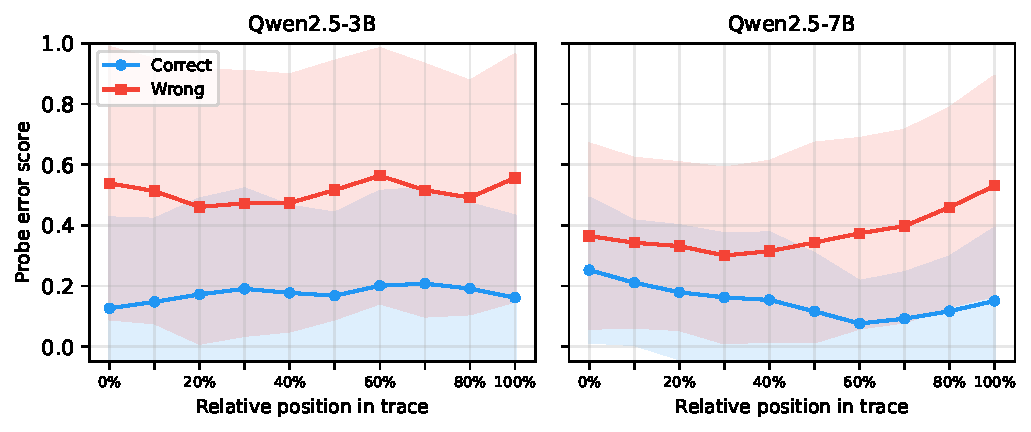
\includegraphics[width=\columnwidth]{fig_step_dynamics.pdf}
\caption{Probe error score trajectories for correct vs.\ wrong traces. \modelsmall{} (left): separation is maximal from Step~1 and stable throughout. \modelmed{} (right): separation grows monotonically, reaching maximum at the final step.}
\label{fig:step_dynamics}
\end{figure}

Figure~\ref{fig:step_dynamics} reveals two distinct error signal patterns.
For \modelsmall, the probe achieves maximum separation at the \textit{very first step} (correct: 0.13 vs.\ wrong: 0.54, gap = 0.41), and this gap persists throughout reasoning.
For \modelmed, the separation starts small (gap = 0.11) but \textit{grows monotonically} to 0.38 by the final step, as correct traces' scores decrease (0.25 $\to$ 0.15) while wrong traces' scores increase (0.36 $\to$ 0.53).

This reveals two regimes: in the smaller model, error detection is ``front-loaded''---the model commits to a flawed trajectory early. In the larger model, error signals accumulate gradually. Both patterns rule out the error signal being a simple post-hoc readout of text quality.

% ============================================================
\section{Reasoning Unfaithfulness}
\label{sec:unfaithful}

The combination of accurate internal error detection and uninformative external signals constitutes \textit{reasoning unfaithfulness}: the model's generated text does not faithfully reflect its internal state.

\subsection{Verbalized Confidence Gap}

We prompt the model to express confidence (1--5 scale) after each trace and compare with probe scores.

\begin{itemize}[leftmargin=*,nosep]
\item \textbf{Correct traces}: verbalized confidence $4.87/5$, mean probe score $0.27$
\item \textbf{Wrong traces}: verbalized confidence $4.55/5$, mean probe score $0.74$
\end{itemize}

The confidence gap is only 0.31 points on a 5-point scale, while the probe score gap is 0.47.
The Spearman correlation between verbalized confidence and probe score is $-0.367$---weak and negative, confirming that text-level confidence carries little information about actual reasoning quality.

\subsection{The Unfaithful Region}

We define a trace as ``unfaithful'' when it simultaneously exhibits high verbalized confidence ($\geq 4$) and high probe error score ($> 0.5$).
Fully 65\% of \textit{wrong} traces fall in this unfaithful region---the model expresses confidence in reasoning that its own hidden states flag as likely wrong.
Only 1\% of traces contain hedging language (``I'm not sure,'' ``let me reconsider'').
Figure~\ref{fig:distributions} shows probe score distributions by correctness: correct and wrong traces are well-separated in the hidden state space but nearly indistinguishable in verbalized confidence.

\begin{figure}[t]
\centering
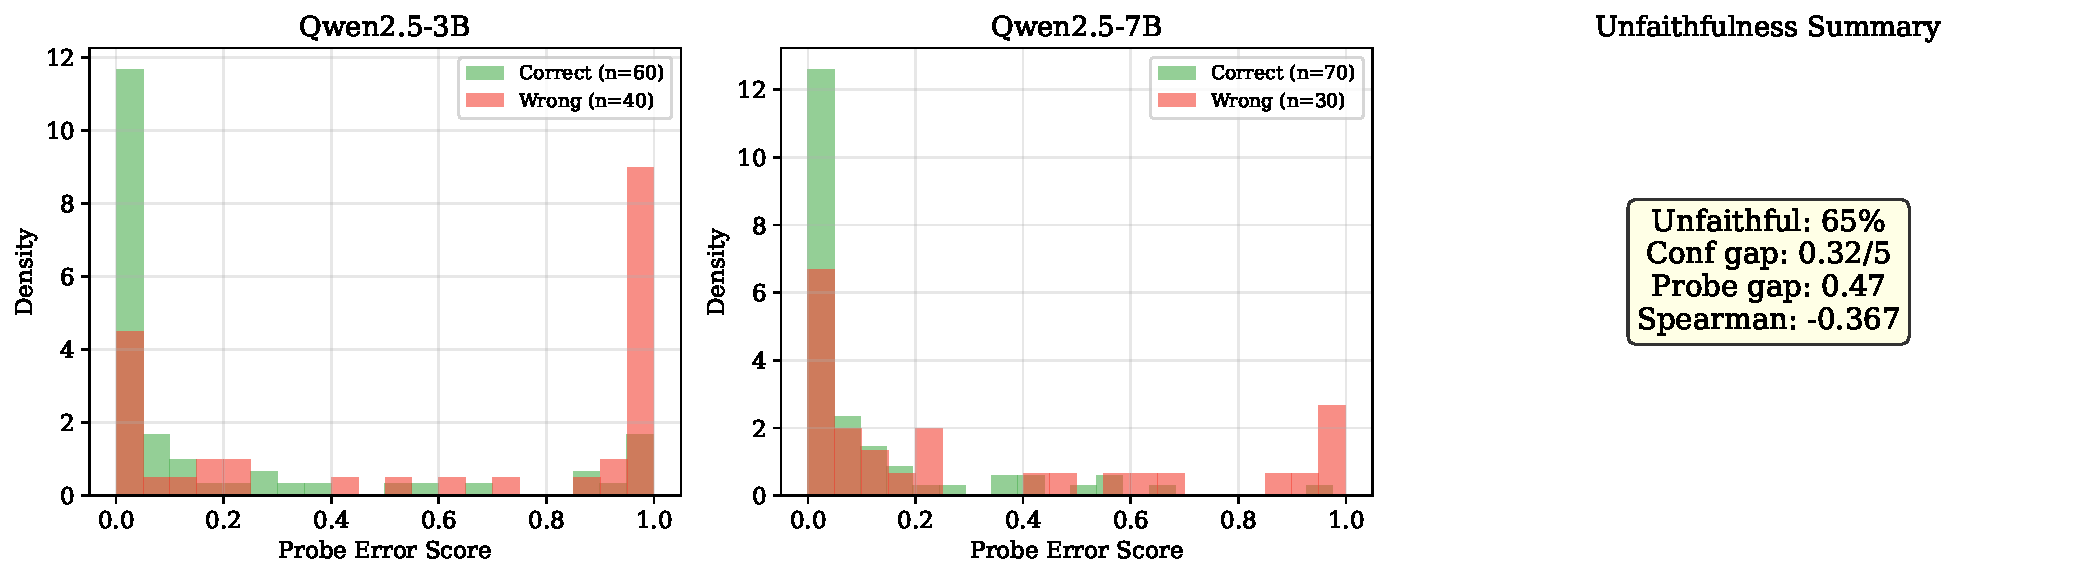
\includegraphics[width=\columnwidth]{fig_probe_distributions.pdf}
\caption{Probe error score distributions for correct vs.\ wrong traces. The probe clearly separates the two populations (left, center panels), while verbalized confidence shows minimal gap (right panel).}
\label{fig:distributions}
\end{figure}

% ============================================================
\section{Intervention Experiments}
\label{sec:interventions}

The preceding sections establish that models internally detect errors with high accuracy.
A natural question follows: can this signal be leveraged to improve reasoning?
We evaluate four intervention strategies and find that \textbf{none meaningfully improve accuracy}.

\subsection{Activation Steering}
\label{sec:steering}

Following representation engineering \cite{zou2023representation}, we extract the probe's weight vector $\mathbf{w}$ as the ``error direction'' and subtract it from hidden states during generation:
\begin{equation}
\mathbf{h}' = \mathbf{h} - \alpha \cdot (\mathbf{h} \cdot \hat{\mathbf{w}}) \cdot \hat{\mathbf{w}}
\end{equation}
where $\hat{\mathbf{w}} = \mathbf{w}/\|\mathbf{w}\|$ and $\alpha$ controls steering strength.

\begin{table}[t]
\centering
\small
\begin{tabular}{lcccc}
\toprule
& \multicolumn{2}{c}{\textbf{\modelsmall}} & \multicolumn{2}{c}{\textbf{\modelmed}} \\
\cmidrule(lr){2-3} \cmidrule(lr){4-5}
$\alpha$ & Acc & $\Delta$ & Acc & $\Delta$ \\
\midrule
0 (base) & 0.53 & --- & 0.60 & --- \\
0.5 & 0.56 & +0.03 & 0.60 & 0.00 \\
1.0 & 0.55 & +0.02 & 0.61 & +0.01 \\
2.0 & 0.55 & +0.02 & 0.62 & +0.02 \\
5.0 & 0.56 & +0.03 & 0.60 & 0.00 \\
8.0 & 0.47 & $-$0.06 & 0.64 & +0.04 \\
\bottomrule
\end{tabular}
\caption{Activation steering results. Gains are modest (+2--4\%) and aggressive steering ($\alpha=8$) can degrade the smaller model.}
\label{tab:steering}
\end{table}

Table~\ref{tab:steering} shows that activation steering provides at most +3\% (3B) and +4\% (7B) improvement.
Aggressive steering degrades performance for the smaller model, suggesting the error direction is primarily \textit{diagnostic} rather than \textit{prescriptive}---removing the error component does not produce correct reasoning.

\subsection{Probe-Guided Best-of-N}

We generate $N$ traces per problem (temperature $= 0.7$) and select the one with the lowest probe error score.

\begin{table}[t]
\centering
\small
\begin{tabular}{lccccc}
\toprule
$N$ & Greedy & Random & MV & Probe & Oracle \\
\midrule
\multicolumn{6}{c}{\textit{\modelsmall}} \\
3 & .60 & .59 & .63 & .58 & .73 \\
8 & .60 & .60 & .67 & .63 & .84 \\
12 & .60 & .56 & \textbf{.75} & .62 & .88 \\
\midrule
\multicolumn{6}{c}{\textit{\modelmed}} \\
3 & .70 & .71 & .71 & .71 & .84 \\
8 & .70 & .70 & \textbf{.76} & .73 & .91 \\
12 & .70 & .72 & \textbf{.75} & .70 & .91 \\
\bottomrule
\end{tabular}
\caption{Probe-guided best-of-N vs.\ baselines. MV = majority vote. The probe fails to outperform majority vote despite large oracle headroom.}
\label{tab:bon}
\end{table}

Table~\ref{tab:bon} reveals that probe-guided selection performs comparably to random selection and substantially underperforms majority vote.
The oracle upper bound (88--91\% at $N$=12) confirms that correct traces exist among candidates---the bottleneck is \textit{selection quality}, and the probe's error score is insufficient for this purpose.

\subsection{Probe-Triggered Self-Correction}

We use the probe to detect likely errors, then prompt the model to ``verify and correct'' its own solution.

\begin{table}[t]
\centering
\small
\begin{tabular}{lcc}
\toprule
\textbf{Strategy} & \textbf{\modelsmall} & \textbf{\modelmed} \\
\midrule
Greedy (no retry) & 0.60 & 0.70 \\
Always retry & 0.57 ($-$3\%) & 0.67 ($-$3\%) \\
Best-of-two (probe) & 0.60 & 0.70 \\
Oracle-triggered & 0.61 (+1\%) & 0.71 (+1\%) \\
\bottomrule
\end{tabular}
\caption{Self-correction results. Retry \textit{degrades} accuracy; even oracle-triggered correction gains only +1\%.}
\label{tab:self_correction}
\end{table}

Table~\ref{tab:self_correction} shows the most striking result: self-correction \textit{actively hurts} accuracy ($-3\%$ for both models).
Even when we use an oracle to retry \textit{only} problems the model actually got wrong, the gain is merely +1\%.
The model cannot meaningfully improve its reasoning through self-correction, regardless of whether the trigger is the probe or an oracle.

\subsection{Causal Analysis: Activation Patching}
\label{sec:patching}

The above experiments show that the error signal cannot be leveraged for self-improvement, but a deeper question remains: is this signal \textit{causally} related to the reasoning process, or merely a diagnostic readout?

We test this via activation patching \cite{meng2022locating,vig2020investigating} on mixed-outcome problems (where the model sometimes succeeds and sometimes fails on the same problem).
For each such problem, we extract the hidden state from a \textit{correct} trace and patch it into a new generation at the best probe layer.

\begin{table}[t]
\centering
\small
\begin{tabular}{lcc}
\toprule
\textbf{Patching Method} & \textbf{\modelsmall} & \textbf{\modelmed} \\
\midrule
Baseline (no patch) & 0.65 & 0.33 \\
Replace with correct HS & 0.35 & 0.33 \\
Blend ($\alpha$=0.3) & 0.52 & 0.20 \\
Blend ($\alpha$=0.5) & 0.00 & 0.07 \\
Subtract error ($\alpha$=0.5) & 0.65 & 0.47 \\
Subtract error ($\alpha$=2.0) & 0.61 & 0.47 \\
\bottomrule
\end{tabular}
\caption{Activation patching on mixed-outcome problems ($n$=23 for 3B, $n$=15 for 7B). Replacing or blending hidden states \textit{degrades} accuracy; subtracting the error direction has no reliable benefit.}
\label{tab:patching}
\end{table}

Table~\ref{tab:patching} provides direct causal evidence: \textbf{patching correct hidden states into new generations does not help---and often catastrophically hurts accuracy}.
Blending at $\alpha$=0.5 reduces 3B accuracy to 0\%.
Even the gentler ``subtract error direction'' intervention produces no reliable gain.

This confirms that the error signal is a \textbf{diagnostic readout, not a causal lever}.
The model's hidden states encode \textit{awareness} of reasoning quality, but this awareness does not reside in a component that can be surgically replaced to redirect computation.

\subsection{Discussion: Why Interventions Fail}

These results collectively reveal that the error signal is \textbf{diagnostic, not prescriptive}.
The model \textit{knows} it is (or will be) wrong, but this knowledge is encoded in a form that does not causally influence reasoning quality.
Activation steering removes the ``error component'' but does not inject ``correct reasoning''---the two are not opposites in representation space.
Self-correction fails because the model generates corrections using the same flawed computation.
Activation patching confirms the signal is a readout, not a control channel.

This asymmetry---\textit{error detection without error correction}---is a core characteristic of reasoning unfaithfulness.
Figure~\ref{fig:interventions} summarizes the intervention strategies.

\begin{figure*}[t]
\centering
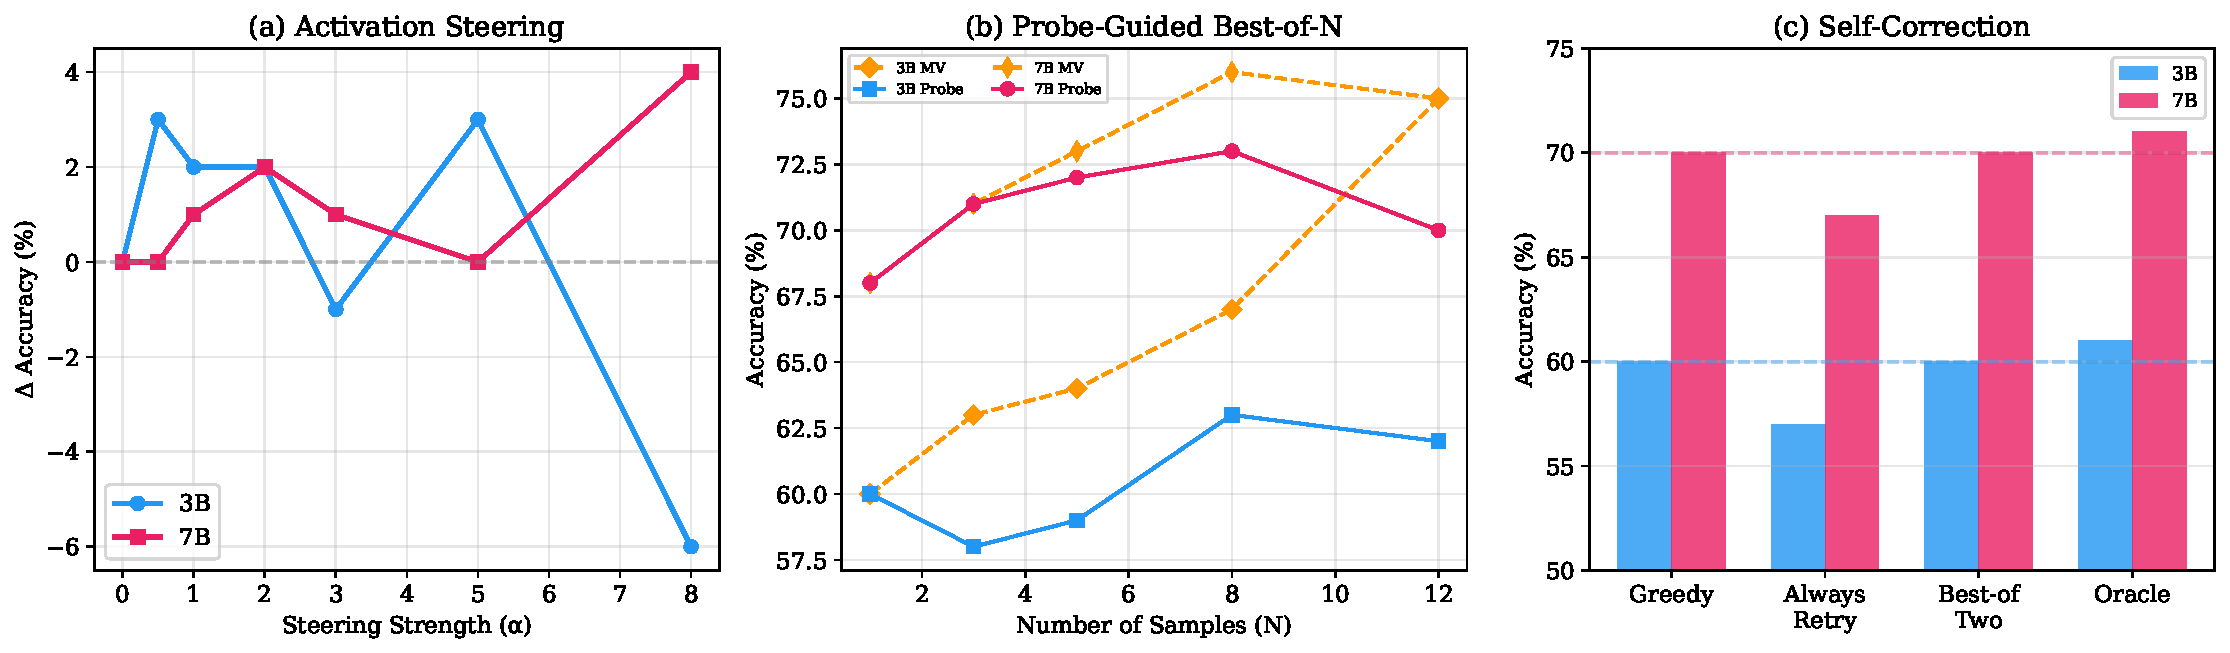
\includegraphics[width=\textwidth]{fig_solution_summary.pdf}
\caption{Summary of intervention experiments. (a) Activation steering provides marginal gains that degrade at high strength. (b) Probe-guided best-of-N underperforms majority vote despite large oracle headroom. (c) Self-correction hurts accuracy for both models; even oracle-triggered retry gains only +1\%.}
\label{fig:interventions}
\end{figure*}

% ============================================================
\section{Selective Routing}
\label{sec:routing}

While internal interventions fail, the probe's error detection capability enables a practical application: \textit{selective routing} to external verification.

\subsection{Method}

Given a trigger rate $r \in (0, 1)$:
\begin{enumerate}[leftmargin=*,nosep]
\item Generate a greedy CoT trace for each problem
\item Score each trace with the probe
\item Route the top-$r$ fraction (by probe score) to an external verifier (GPT-4o-mini)
\item Keep original answers for the remaining $1-r$ fraction
\end{enumerate}

\subsection{Results}

\begin{table}[t]
\centering
\small
\begin{tabular}{lcccc}
\toprule
\textbf{Method} & \textbf{Acc} & \textbf{$\Delta$} & \textbf{API calls} \\
\midrule
Baseline (\modelsmall) & 0.53 & --- & 0\% \\
Always API & 0.57 & +0.04 & 100\% \\
Random routing (40\%) & 0.56 & +0.03 & 40\% \\
\textbf{Probe routing (40\%)} & \textbf{0.61} & \textbf{+0.08} & \textbf{40\%} \\
Probe routing (60\%) & 0.61 & +0.08 & 60\% \\
\bottomrule
\end{tabular}
\caption{Selective routing results. Probe-guided routing at 40\% achieves +8\% accuracy, exceeding always-API (+4\%) at less than half the compute cost.}
\label{tab:routing}
\end{table}

Table~\ref{tab:routing} shows that probe-guided routing achieves \textbf{+8\% accuracy at 40\% API cost}, \textit{exceeding} the always-API strategy (+4\%).
This super-additive effect occurs because always-API routing is a double-edged sword: the external verifier fixes 11 wrong traces but \textit{also breaks 7 correct ones} (on $n$=100).
Probe routing avoids this by preserving correct answers and targeting API effort exclusively on likely errors.

When we replace external routing with self-retry (same model), gains drop to +1--2\%, again confirming that the bottleneck is \textit{correction capability}, not error detection.
For comparison, using GPT-4o-mini as a step-by-step LLM monitor (checking each step during generation) achieves similar accuracy but requires 9$\times$ more tokens---the probe provides equivalent error detection at negligible cost.
Figure~\ref{fig:routing} shows the full refinement curve.

\paragraph{Probe + majority vote hybrid.}
An alternative to external routing is using the probe to selectively apply majority vote (MV)---an expensive but API-free strategy.
We generate $N$=8 samples per problem and apply MV only to the top-$r$ fraction flagged by the probe, keeping greedy answers for the rest.
Full MV improves accuracy from 0.49 to 0.59 (+10\%) at 8$\times$ compute cost.
However, probe-guided selective MV provides \textit{no meaningful advantage} over random selection: at 40\% rate, both achieve 0.54 (cost 3.8$\times$).
This is consistent with the best-of-N finding (Table~\ref{tab:bon}): the probe reliably detects \textit{that} a trace is wrong but cannot improve \textit{selection among alternatives}.
External routing succeeds precisely because it brings in a qualitatively different computation, not merely more samples from the same model.

\begin{figure}[t]
\centering
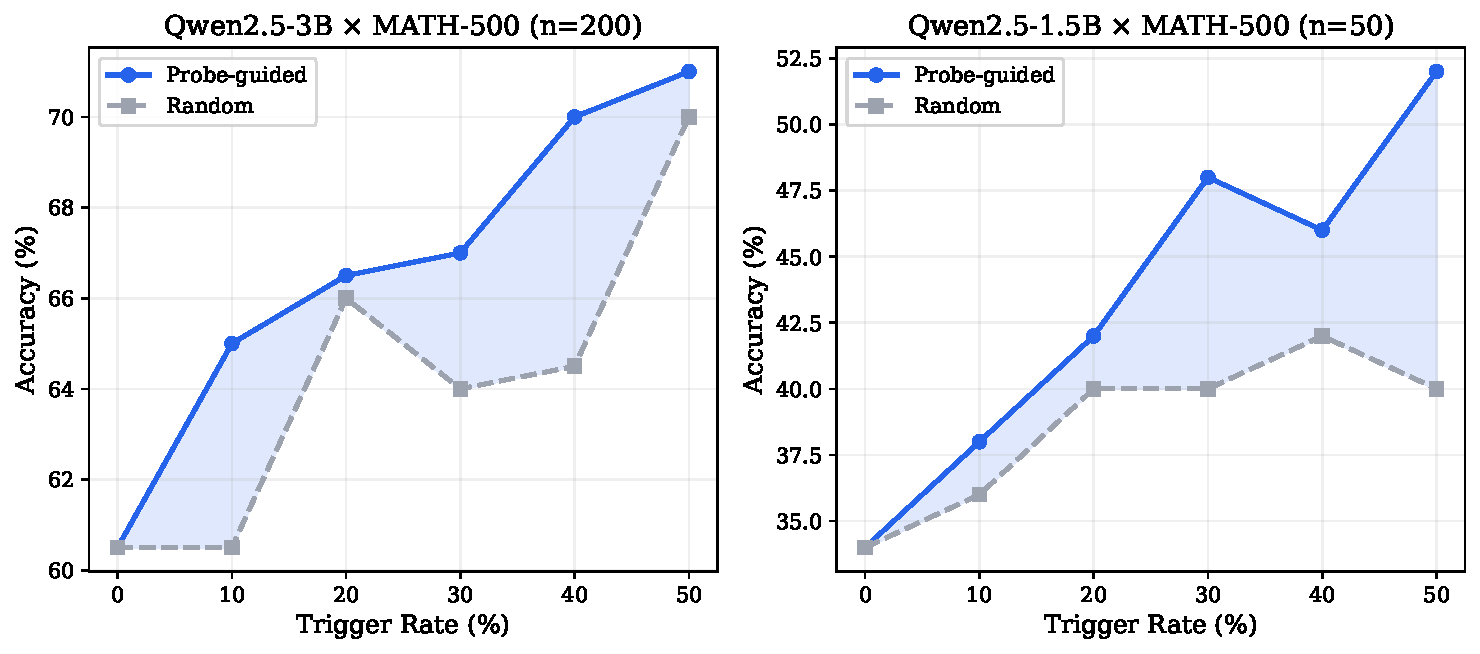
\includegraphics[width=\columnwidth]{fig4_e2e_refinement.pdf}
\caption{Selective refinement: probe-guided vs.\ random trigger at various rates. Probe-guided consistently outperforms random, with the gap widest at moderate trigger rates (30--60\%).}
\label{fig:routing}
\end{figure}

% ============================================================
\section{Discussion}
\label{sec:discussion}

\paragraph{Non-monotonic scaling of probe accuracy.}
Probe AUROC does not decrease monotonically with model scale: it is highest for 72B (0.977), followed by 32B (0.956) and 3B (0.953), but dips at 7B (0.669) and 14B (0.762).
Bootstrap 95\% CIs on held-out data confirm stability (3B: 0.80 [0.70, 0.88]; 7B: 0.76 [0.66, 0.87]; 32B: 0.96 [0.95, 1.00]).
The strong recovery at 32B and 72B demonstrates that hidden error awareness is \textit{not} limited to small models---in fact, it strengthens at larger scale.
The intermediate dip at 7B/14B likely reflects training dynamics: these models make fewer errors that are less systematic, creating a harder linear separation problem.
Consistent with this, within-problem separation (difficulty control) is strongest for 7B ($d = 0.63$) and 3B ($d = 0.55$), and weaker for 14B ($d = 0.13$).
The 72B result, where the probe achieves its highest AUROC despite lower raw accuracy, suggests that larger models develop \textit{more linearly structured} error representations.

\paragraph{Two temporal regimes of error awareness.}
The step dynamics reveal a qualitative difference across scales.
The 3B model shows \textit{front-loaded} error awareness: maximum probe separation at Step~1 (gap = 0.41), suggesting early commitment to a flawed trajectory.
The 7B model shows \textit{accumulating} error awareness: separation grows monotonically from 0.11 to 0.38, suggesting that error signals build as the model processes more reasoning steps.
These two regimes may reflect different failure modes: the 3B model may lack the capacity to represent correct solutions for hard problems (detectable immediately), while the 7B model may begin correctly but drift during extended reasoning.

\paragraph{Why is the signal diagnostic but not causal?}
The probe captures a \textit{summary statistic} of computation quality---analogous to a thermometer reading body temperature---rather than a causal variable determining reasoning outcomes.
Activation patching provides the strongest evidence: replacing hidden states from correct traces does not produce correct reasoning but destroys coherent output.
This is consistent with the view that reasoning quality emerges from distributed, multi-layer computation \cite{meng2022locating}, not from a single layer that could be surgically corrected.

\paragraph{Relation to process reward models.}
Our probe can be viewed as a lightweight, unsupervised process reward model (PRM) \cite{lightman2024lets}: it scores intermediate reasoning steps without requiring step-level labels.
However, unlike PRMs that are trained on large-scale human annotations, our probe requires only 50 problems with binary outcome labels.
The trade-off is that our probe is less accurate for \textit{selection} (it underperforms majority vote in best-of-N), but highly effective for \textit{triage} (identifying which traces need external verification).

% ============================================================
\section{Conclusion}
\label{sec:conclusion}

We have shown that LLMs internally detect their reasoning errors with high accuracy (up to 0.95 AUROC) while generating text that conceals this knowledge---a phenomenon we term \textit{hidden error awareness}.
The signal emerges from the very first reasoning step, before any error appears in text, and persists from 1.5B to 72B parameters across model families---strengthening at larger scale---though its temporal profile varies systematically.

Four intervention strategies fail to leverage this signal for self-improvement, revealing that it is diagnostic rather than causal.
The sole effective application is selective routing to external verification, achieving +8\% accuracy at 40\% of full verification cost.

Our findings challenge the assumption that CoT traces faithfully reflect model computation, and suggest that future work on LLM self-correction must address the fundamental asymmetry between error detection and error correction.
The existence of hidden error awareness also opens new directions: can training objectives be designed to make models \textit{act on} their internal error signals rather than merely harboring them?

% ============================================================
\section*{Limitations}

\paragraph{Model scale.} Our experiments span 1.5B--72B parameters across two model families (Qwen, Phi), with probe AUROC \textit{increasing} at larger scale (0.98 for 72B). Whether hidden error awareness persists in frontier models (100B+, closed-source) remains an open question, as our method requires hidden-state access.

\paragraph{Domain scope.} Our primary results use mathematical reasoning (MATH-500). Native ARC probes confirm the phenomenon extends to commonsense reasoning, but cross-domain transfer is limited. Whether similar signals exist in code generation, multi-hop reasoning, or long-context tasks requires further investigation.

\paragraph{Sample sizes.} Activation patching and difficulty control experiments use moderate sample sizes ($n$=13--23 mixed-outcome problems per model). While results are consistent across models, larger-scale replication would strengthen conclusions.

\paragraph{Probe access and external verifier.} Our method requires access to hidden states (unavailable for API-only models) and the routing strategy assumes access to a stronger external verifier.

% ============================================================
\section*{Ethics Statement}

Our work exposes a gap between LLMs' internal representations and their generated text during reasoning.
This has potential dual-use implications: the probe could be used to detect unreliable reasoning (beneficial) but could also inform adversarial attacks that exploit the gap between internal knowledge and surface behavior.
We release our methodology but emphasize that deployment of probe-based systems should include appropriate safeguards.
All experiments use publicly available models and benchmarks; no human subjects were involved.

% ============================================================
\bibliography{references}
\bibliographystyle{acl_natbib}

\clearpage
\appendix

\section{Prompt Templates}
\label{app:prompts}

\paragraph{CoT generation.}
All models use the following system-agnostic prompt wrapped in each model's chat template:
\begin{quote}\small\ttfamily
Solve the following math problem step by step. Number each step as `Step 1:', `Step 2:', etc. End with `ANSWER: <your final answer>'.\\[4pt]
Problem: \{problem\}\\[4pt]
Solution:
\end{quote}

\paragraph{Verbalized confidence.}
After generating a CoT trace, we append:
\begin{quote}\small\ttfamily
Rate your confidence in the above answer on a scale from 1 (very uncertain) to 5 (very confident). Reply with just the number.
\end{quote}

\paragraph{Self-correction.}
For the retry intervention (\S\ref{sec:interventions}):
\begin{quote}\small\ttfamily
Review your solution carefully. If you find any errors, correct them. Provide your final answer after `ANSWER:'.
\end{quote}

\section{Hyperparameters and Training Details}
\label{app:hyperparams}

\begin{table}[h]
\centering
\small
\begin{tabular}{ll}
\toprule
\textbf{Parameter} & \textbf{Value} \\
\midrule
Probe classifier & Logistic Regression \\
Regularization ($C$) & 0.1 ($L_2$) \\
Max iterations & 2000 \\
Feature scaling & StandardScaler (per-dim) \\
CV strategy & 5-fold stratified \\
Training set & 100 MATH-500 problems \\
Generation & Greedy (temp=0) \\
Max new tokens & 512 (CoT), 1024 (full) \\
Hidden state position & Last token of trace \\
\midrule
Best-of-N temperature & 0.7 \\
Best-of-N top-$p$ & 0.95 \\
Steering $\alpha$ range & 0.5, 1.0, 2.0, 5.0, 8.0 \\
Patching $\alpha$ range & 0.3, 0.5 (blend); 0.5, 2.0 (subtract) \\
\midrule
External verifier & GPT-4o-mini \\
Routing threshold & Top-$r$ by probe score \\
\bottomrule
\end{tabular}
\caption{Hyperparameters used across all experiments.}
\label{tab:hyperparams}
\end{table}

\section{Per-Layer Probe Results}
\label{app:layers}

\begin{table}[h]
\centering
\small
\begin{tabular}{lccccc}
\toprule
\textbf{Model} & \textbf{Layers} & \textbf{Best} & \textbf{AUROC} & \textbf{Depth \%} \\
\midrule
Qwen2.5-1.5B & 28 & 27 & 0.918 & 96\% \\
\modelsmall & 36 & 27 & 0.953 & 75\% \\
\modelphi & 32 & 8 & 0.936 & 25\% \\
\modelmed & 28 & 16 & 0.669 & 57\% \\
\modellarge & 48 & 39 & 0.762 & 81\% \\
Qwen2.5-32B & 64 & 32 & 0.956 & 50\% \\
Qwen2.5-72B & 80 & 64 & 0.977 & 80\% \\
\bottomrule
\end{tabular}
\caption{Best probe layer by model. Depth \% = best layer / total layers. Upper-half layers consistently yield the strongest signal.}
\label{tab:layer_details}
\end{table}

\section{Probe + Majority Vote Hybrid}
\label{app:hybrid}

Table~\ref{tab:hybrid} shows the full results of the probe + majority vote hybrid experiment (\S\ref{sec:routing}).

\begin{table}[h]
\centering
\small
\begin{tabular}{rcccc}
\toprule
\textbf{Rate} & \textbf{Probe+MV} & \textbf{Random+MV} & \textbf{$\Delta$ vs.\ random} & \textbf{Cost} \\
\midrule
10\% & 0.49 & 0.49 & 0.00 & 1.7$\times$ \\
20\% & 0.50 & 0.50 & 0.00 & 2.4$\times$ \\
30\% & 0.52 & 0.53 & $-$0.01 & 3.1$\times$ \\
40\% & 0.54 & 0.54 & 0.00 & 3.8$\times$ \\
50\% & 0.54 & 0.54 & 0.00 & 4.5$\times$ \\
60\% & 0.55 & 0.54 & +0.01 & 5.2$\times$ \\
80\% & 0.58 & 0.57 & +0.01 & 6.6$\times$ \\
100\% & 0.59 & 0.59 & 0.00 & 8.0$\times$ \\
\bottomrule
\end{tabular}
\caption{Probe + MV hybrid vs.\ random + MV on \modelsmall{} ($N$=8 samples, $n$=100 problems). Greedy baseline: 0.49, full MV: 0.59. The probe provides no meaningful advantage over random selection for MV targeting.}
\label{tab:hybrid}
\end{table}

\end{document}
